\graphicspath{{chapters/software/}}


\chapter{CCA-Zoo: A collection of Regularized, Deep Learning-based, Kernel, and Probabilistic methods in a scikit-learn style framework}\label{ch:software}

% \epigraph{And that's really the essence of programming. By the time you've sorted out a complicated idea into little steps that even a stupid machine can deal with, you've learned something about it yourself.}{\textit{Douglas Adams}}
\minitoc
\section*{Preface}

This work was published in the Journal of Open Source Software \citep{chapman2021cca}.
I have been the lead developer of the \texttt{CCA-Zoo} package since its inception in 2020.
All of the methods we have described in this thesis are implemented in \texttt{CCA-Zoo} and are immediately available for use by the research community.

\section{Introduction}

This chapter presents \texttt{CCA-Zoo}, a comprehensive Python library for multiview learning that was developed as a key contribution of this thesis. \texttt{CCA-Zoo} brings together a wide range of methods for canonical correlation analysis (CCA), partial least squares (PLS), and related techniques, providing efficient and user-friendly implementations that integrate seamlessly with the Python data science ecosystem.

The development of \texttt{CCA-Zoo} was motivated by the recognition that the lack of well-developed and widely available software has been a major barrier to the adoption and advancement of multiview learning methods, particularly in the Python community. While popular libraries like \texttt{scikit-learn} \citep{pedregosa2011scikit} offer basic implementations of classical techniques like CCA and PLS, they lack support for many of the important extensions and variants that have been proposed in the literature to handle challenges such as high-dimensional data, non-linearity, sparsity, and deep learning.

\texttt{CCA-Zoo} aims to fill this gap by providing a unified framework for multiview learning that is both comprehensive and accessible. The library includes implementations of both classical and state-of-the-art methods, ranging from regularized and kernel-based extensions of CCA and PLS to modern deep learning and probabilistic approaches. These implementations are designed to be efficient, scalable, and easy to use, with a consistent API that follows the conventions of \texttt{scikit-learn}.

In addition to its core algorithms, \texttt{CCA-Zoo} provides a range of tools and utilities to support the entire multiview learning workflow, from data preprocessing and feature selection to model evaluation and visualization. The library also includes a collection of example datasets and pre-trained models, making it easy for users to get started and explore different techniques on real-world problems.

Throughout the development of this thesis, \texttt{CCA-Zoo} has played a central role as both a research tool and a means of disseminating our methodological contributions to the wider community. The experiments and case studies presented in the previous chapters have all relied on \texttt{CCA-Zoo} implementations, ensuring reproducibility and comparability of our results. At the same time, by releasing \texttt{CCA-Zoo} as an open-source library on GitHub and PyPi, we have enabled other researchers and practitioners to easily build upon and extend our work.

We also discuss the impact that \texttt{CCA-Zoo} has had so far, both within the context of this thesis and in the broader research community, and outline directions for future development and improvement. Our hope is that \texttt{CCA-Zoo} will serve as a valuable resource and catalyst for advancing the state-of-the-art in multiview learning, and for bridging the gap between methodological research and practical application.

\section{Background: Software for Multiview Learning}

The field of multiview learning has recently witnessed a surge of interest from the research community. This growth can be attributed to the increasing availability of multi-modal data across various domains, from bioinformatics to social media analysis, and the recognition that integrating multiple views can often lead to better insights and predictions than relying on a single perspective.

Traditionally, the development of multiview learning methods has been dominated by researchers in the statistical learning community, who have primarily relied on programming languages like R and MATLAB. These platforms have served as fertile ground for the creation and dissemination of many state-of-the-art algorithms.

However, this has created a challenge for researchers and practitioners who prefer to work in the Python programming language, which has become increasingly popular for machine learning tasks due to its simplicity, flexibility, and rich ecosystem of libraries. Python users have been faced with two suboptimal options: either port existing R or MATLAB implementations into Python, which can be a time-consuming and error-prone process requiring significant domain expertise, or make do with the limited set of multiview methods available in general-purpose Python libraries like \texttt{scikit-learn} \citep{pedregosa2011scikit}.

This fragmentation of the multiview learning landscape across different programming languages has created significant barriers to entry for Python users, potentially hindering the widespread adoption and application of these powerful techniques. Moreover, it has made it difficult for researchers to compare and benchmark different methods on a level playing field, as implementations may vary widely in terms of performance, scalability, and ease of use.

The \texttt{CCA-Zoo} package aims to address these challenges by providing a comprehensive and unified platform for multiview learning in Python. By offering a wide range of algorithms spanning both classical and state-of-the-art approaches, \texttt{CCA-Zoo} enables researchers and practitioners to easily explore and apply these techniques to their own data and problems, without the need for extensive domain expertise or cumbersome porting of code.

Through its scikit-learn compatible API, modular design, and efficient implementations, \texttt{CCA-Zoo} seamlessly integrates with the existing Python machine learning ecosystem, lowering the barriers to entry and accelerating the pace of research and application in multiview learning. By bringing together methods from different research communities and programming languages under a common framework, \texttt{CCA-Zoo} also facilitates fair and reproducible comparisons of different approaches, helping to advance our understanding of their strengths and limitations.

In the following sections, we will consider the design principles, key features, and implementation details of \texttt{CCA-Zoo}, showcasing how it can be used to streamline and enhance multiview learning workflows in Python.

\section{Methods: Design and Implementation of \texttt{CCA-Zoo}}

\texttt{CCA-Zoo} is designed to be a comprehensive and user-friendly library for multiview learning in Python. In this section, we describe the key design decisions and implementation details that underpin its functionality, flexibility, and performance. Figure \ref{fig:cca-zoo-api} provides an overview of the library's structure and its integration with the wider Python machine learning ecosystem.

\subsection{API Design and Scikit-Learn Compatibility}

A central goal in the development of \texttt{CCA-Zoo} was to ensure maximum compatibility and interoperability with the existing Python machine learning ecosystem. To this end, we adopted the API design principles and conventions of the widely-used \texttt{scikit-learn} library \citep{pedregosa2011scikit}. \texttt{Scikit-learn} has become the de facto standard for machine learning in Python, thanks to its consistent, user-friendly API and its extensive collection of tools for data preprocessing, model selection, evaluation, and visualization.

By adhering to the \texttt{scikit-learn} API, \texttt{CCA-Zoo} inherits these benefits and ensures that users can seamlessly integrate multiview learning methods into their existing workflows. All estimators in \texttt{CCA-Zoo} follow the fit-transform pattern, where the \texttt{fit()} method learns model parameters from training data, and the \texttt{transform()} method applies the learned transformation to new data. Hyperparameters are specified as constructor arguments, allowing easy model creation and configuration.

This design choice not only makes \texttt{CCA-Zoo} intuitive and easy to use for anyone familiar with \texttt{scikit-learn}, but also enables the use of \texttt{scikit-learn}'s powerful model selection and evaluation tools, such as cross-validation and grid search, directly with \texttt{CCA-Zoo} estimators. Users can construct complex pipelines that include data preprocessing, feature selection, and multiview learning steps, all with a consistent, declarative syntax.

Figure \ref{fig:cca-zoo-api} illustrates this integration, highlighting \texttt{CCA-Zoo}'s compatibility with key components of the Python machine learning stack.

\begin{figure}[ht]
\centering
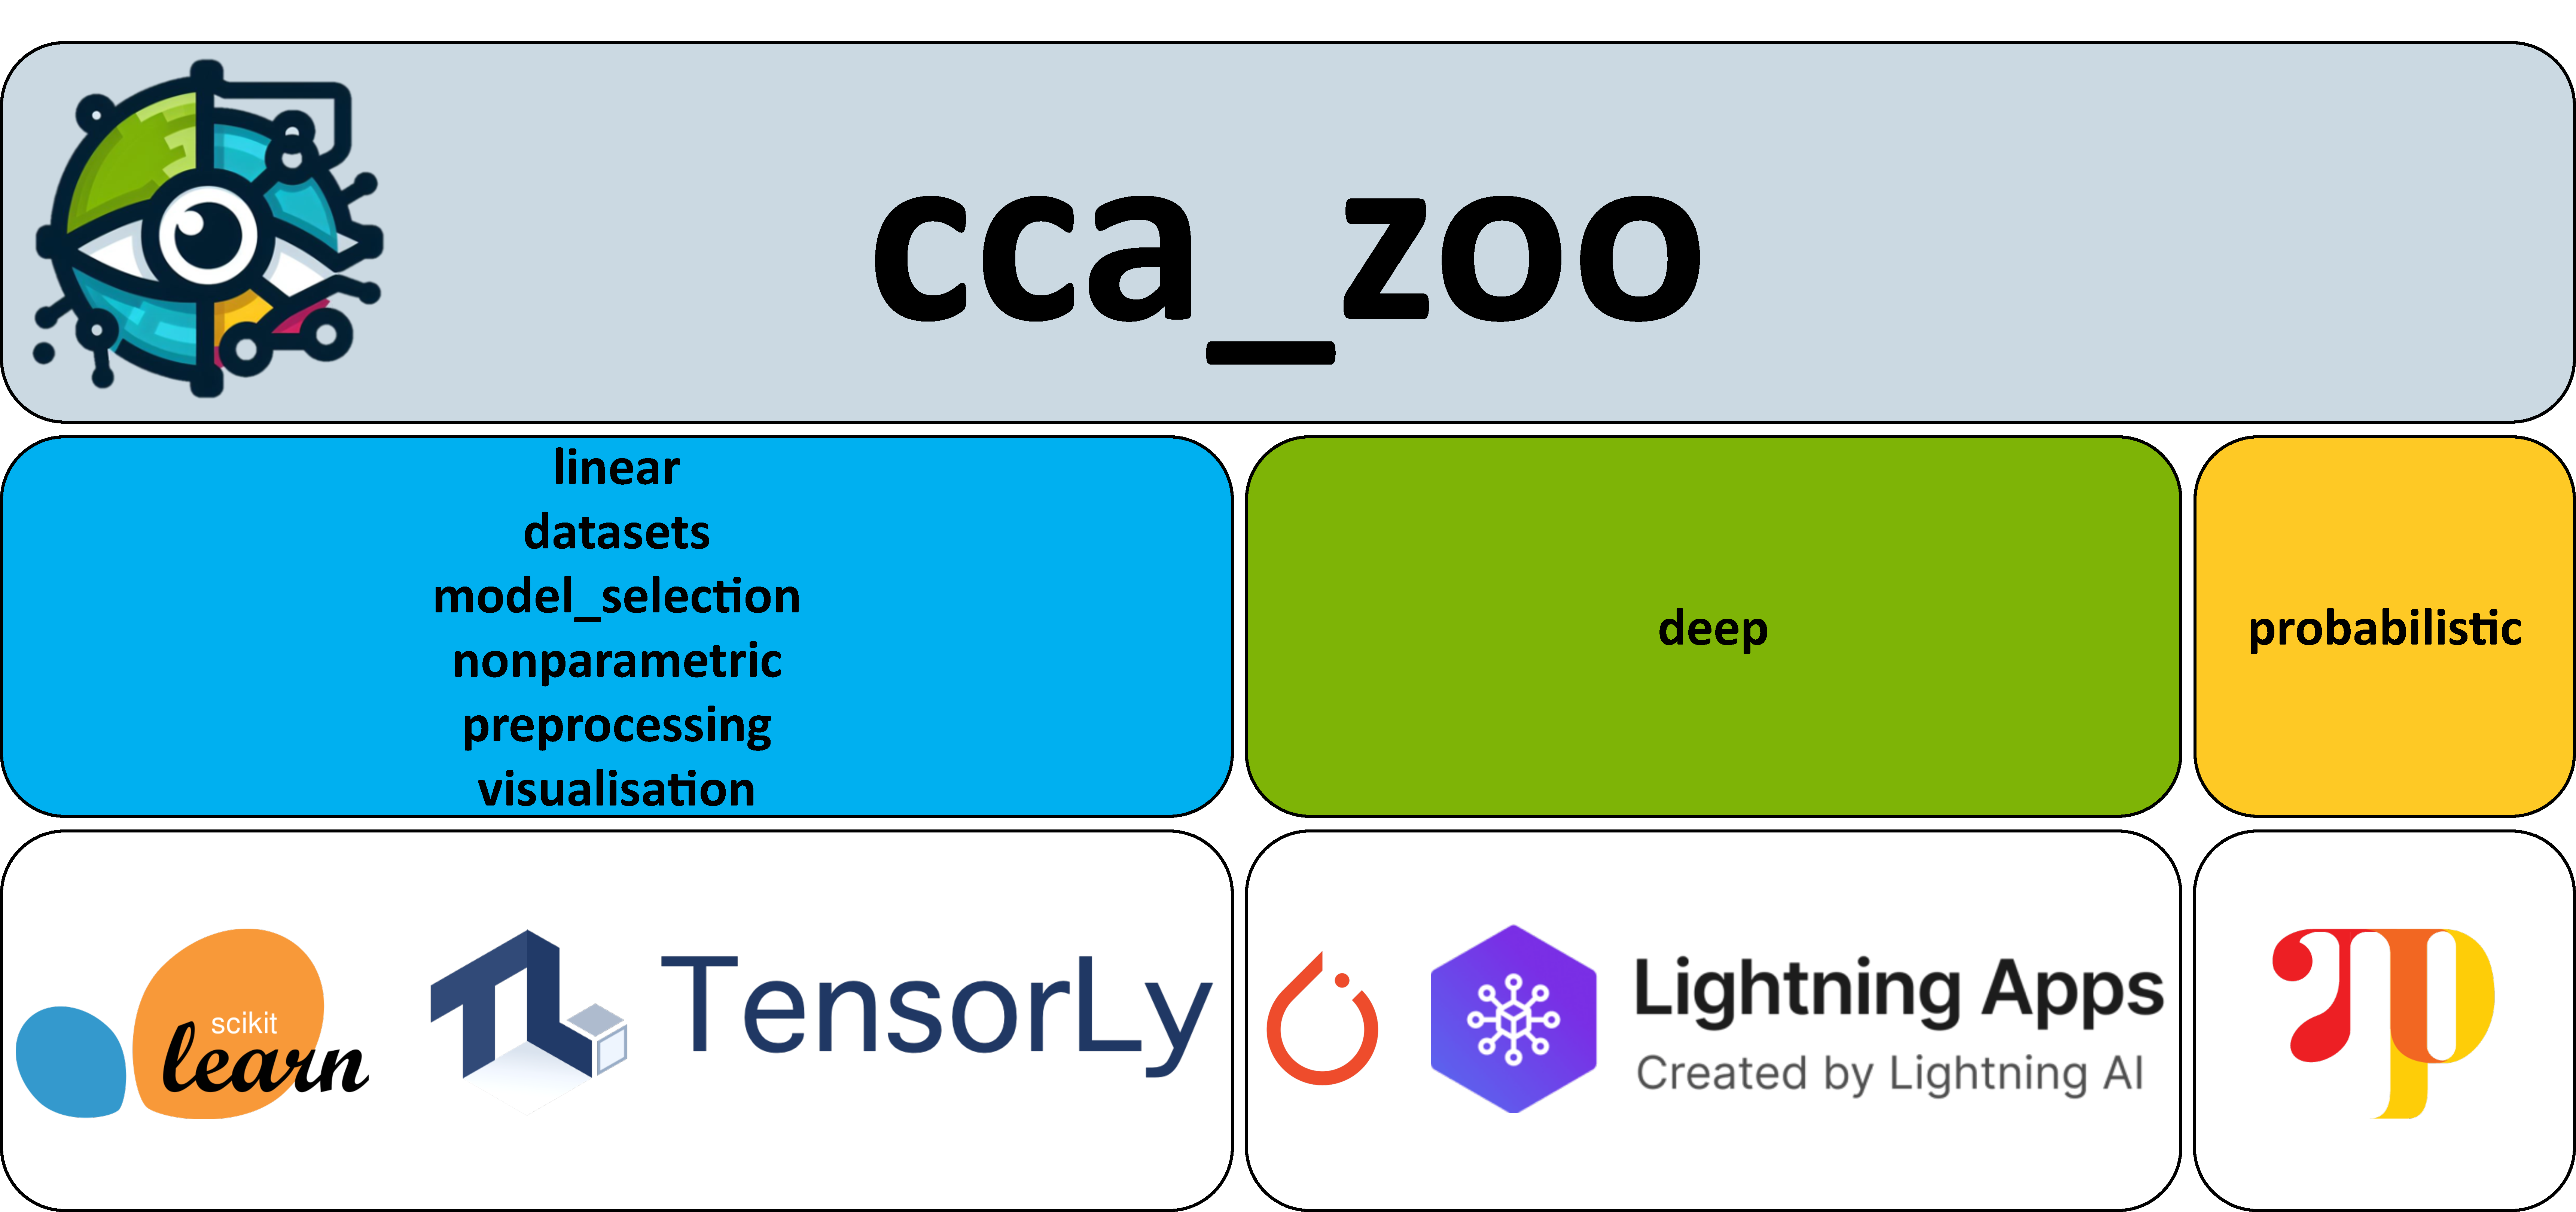
\includegraphics[width=0.8\textwidth]{figures/CCA_Zoo_map}
\caption[The \texttt{CCA-Zoo} compatibility map]{The \texttt{CCA-Zoo} compatibility map showcases integration with various machine learning packages. The deep learning module is built upon \texttt{PyTorch} and \texttt{Lightning}, reflecting their status as industry standards for neural network implementations. The probabilistic module employs \texttt{NumPyro} for its Bayesian inference capabilities, enhancing the application of probabilistic approaches in CCA.}
\label{fig:cca-zoo-api}
\end{figure}

\subsection{Modular Architecture and Extensibility}

Another key design principle of \texttt{CCA-Zoo} is modularity. The library is organized into distinct submodules, each focusing on a specific aspect of the multiview learning workflow:

\begin{itemize}
\item \texttt{datasets}: Classes for generating synthetic data and loading real-world datasets.
\item \texttt{preprocessing}: Tools for data normalization, scaling, and dimensionality reduction.
\item \texttt{model\_selection}: Wrappers for \texttt{scikit-learn}'s cross-validation and hyperparameter tuning utilities, adapted for multiview settings.
\item \texttt{linear}: Estimators for linear CCA, PLS, and their variants.
\item \texttt{deep}: Deep learning-based approaches, built on top of \texttt{PyTorch} \citep{paszke2019pytorch} and \texttt{PyTorch Lightning} \citep{falcon2019pytorch}.
\item \texttt{probabilistic}: Bayesian multiview learning methods, implemented with \texttt{NumPyro} \citep{phan2019composable}, a probabilistic programming library built on top of \texttt{JAX} \citep{deepmind2020jax}.
\item \texttt{visualization}: Functions for visualizing model parameters, latent spaces, and performance metrics.
\end{itemize}

This modular structure makes the codebase more maintainable and easier to navigate. It also facilitates extensibility: new methods and features can be added to each submodule without affecting the rest of the library, as long as they adhere to the common API conventions.

Furthermore, the use of well-established libraries like \texttt{PyTorch}, \texttt{PyTorch Lightning}, and \texttt{NumPyro} for the deep learning and probabilistic modules ensures that \texttt{CCA-Zoo} can benefit from the latest advancements in these rapidly evolving fields. Developers can easily experiment with new architectures, loss functions, and inference techniques, while still leveraging the data handling and model evaluation capabilities of the core \texttt{CCA-Zoo} framework.

\subsection{Flexibility and Ease of Use}

\texttt{CCA-Zoo} is designed to be flexible and easy to use for a wide range of multiview learning tasks. The library provides a unified interface for working with both linear and nonlinear methods, unsupervised and semi-supervised settings, and two-view and multi-view scenarios.

The choice of default hyperparameters and architectural choices for deep learning models has been carefully considered to ensure good performance on a variety of datasets without the need for extensive tuning. At the same time, users have full control over these settings and can easily customize them for specific tasks.

\texttt{CCA-Zoo} also includes a range of utility functions and classes that simplify common tasks and help users avoid boilerplate code. For example, the \texttt{datasets} module provides a consistent interface for accessing and sampling from both synthetic and real-world datasets, handling data loading, splitting, and formatting behind the scenes.

Similarly, the \texttt{model\_selection} module extends \texttt{scikit-learn}'s cross-validation and grid search tools to handle the multi-view setting seamlessly. Users can perform model selection and hyperparameter tuning with just a few lines of code, without having to worry about the intricacies of indexing and reshaping views.

Listing \ref{lst:cca-zoo-example} demonstrates this simplicity and flexibility, showing a complete workflow for training and evaluating a regularized CCA model with cross-validated hyperparameter selection:

% Indent the listing to the right
\begin{listing}[ht]
\begin{minted}{python}
from cca_zoo.datasets import LatentVariableData
from cca_zoo.linear import rCCA
from cca_zoo.model_selection import GridSearchCV
from cca_zoo.visualisation import SeparateRepresentationScatterDisplay

#Generate synthetic multi-view data
data = LatentVariableData(view_features=[10, 10], latent_dims=2)
X, Y = data.sample(n_samples=200, seed=42)

#Define hyperparameter grid
param_grid = {
'c': ([0.1, 0.3, 0.7, 0.9], [0.1, 0.3, 0.7, 0.9]),
}

#Perform cross-validated grid search
model = GridSearchCV(rCCA(latent_dimensions=2),
param_grid=param_grid,
cv=5).fit(X, Y)

#Visualize latent space
SeparateRepresentationScatterDisplay.from_estimator(model.best_estimator_)
\end{minted}
\caption{A complete example of training and evaluating a regularized CCA model with \texttt{CCA-Zoo}.}
\label{lst:cca-zoo-example}
\end{listing}

This example showcases several key features of \texttt{CCA-Zoo}:

\begin{itemize}
\item The \texttt{LatentVariableData} class allows easy generation of synthetic multi-view data with a specified number of features and latent dimensions.
\item The \texttt{rCCA} class provides a regularized CCA estimator with a \texttt{scikit-learn}-compatible API, supporting both fit-transform and inverse transform operations.
\item The \texttt{GridSearchCV} class wraps \texttt{scikit-learn}'s grid search functionality, automatically handling the multi-view parameter grid and cross-validation splitting.
\item The \texttt{SeparateRepresentationScatterDisplay} class provides a high-level interface for visualizing the learned latent space, with separate plots for each view.
\end{itemize}

By providing such high-level abstractions and adhering to familiar API conventions, \texttt{CCA-Zoo} aims to make multiview learning methods accessible to a wide audience, from seasoned machine learning practitioners to domain experts in fields like bioinformatics, computer vision, and natural language processing.

\subsection{Performance and Scalability}

In addition to ease of use and flexibility, \texttt{CCA-Zoo} is designed with performance and scalability in mind. The library is implemented in pure Python, with computationally intensive operations delegated to optimized libraries like \texttt{NumPy} \citep{harris2020array}, \texttt{SciPy} \citep{virtanen2020scipy}, and \texttt{PyTorch}.

For linear methods like CCA and PLS, \texttt{CCA-Zoo} leverages the randomized SVD and other matrix approximation techniques to efficiently handle high-dimensional data. These techniques allow the library to scale to datasets with millions of features and samples, without sacrificing accuracy or numerical stability.

In the deep learning module, \texttt{CCA-Zoo} takes advantage of PyTorch's GPU acceleration and automatic differentiation capabilities to enable fast training of complex models on large-scale datasets. The use of \texttt{PyTorch Lightning} further streamlines the training process, providing a high-level interface for distributed training, checkpointing, and logging.

For probabilistic methods, \texttt{CCA-Zoo} leverages the power of \texttt{NumPyro} and \texttt{JAX} to perform efficient variational inference and MCMC sampling on both CPUs and GPUs. The use of modern probabilistic programming techniques allows users to easily specify and train complex Bayesian models, while still benefiting from the performance and scalability of the underlying libraries.

\texttt{CCA-Zoo}'s performance and scalability claims are backed by extensive benchmarking and testing on a variety of synthetic and real-world datasets. In Section \ref{sec:experiments}, we present a selection of these experiments, comparing \texttt{CCA-Zoo}'s performance to other popular multiview learning libraries and demonstrating its ability to handle large-scale, high-dimensional data.

\subsection{Development and Maintenance}

\texttt{CCA-Zoo} is developed as an open-source project, with its source code and documentation hosted on GitHub at \url{https://github.com/jameschapman19/cca_zoo}. The library follows modern software development best practices, including version control, continuous integration, and automated testing.

The development team is committed to maintaining and improving \texttt{CCA-Zoo} over the long term. This includes fixing bugs, adding new features and methods, and keeping dependencies up to date. The team also welcomes contributions from the community in the form of bug reports, feature requests, and pull requests.

To ensure the library's quality and reliability, \texttt{CCA-Zoo} includes a comprehensive test suite that covers all major functionality. These tests are automatically run on each commit and pull request, using continuous integration services like Travis CI and GitHub Actions. This helps catch regressions and ensures that new features are properly integrated and documented.

\texttt{CCA-Zoo}'s documentation is another key aspect of its maintenance and development. The library includes extensive API documentation, generated automatically from docstrings using tools like Sphinx and Read the Docs. The documentation also includes user guides, tutorials, and examples to help users get started and make the most of the library's features.

In addition to the API documentation, \texttt{CCA-Zoo}'s GitHub repository includes a wiki and issue tracker where users can find additional information, ask questions, and report bugs. The development team is responsive to user feedback and strives to address issues in a timely manner.

By adhering to these development and maintenance practices, \texttt{CCA-Zoo} aims to provide a stable, reliable, and well-documented library that can serve as a foundation for multiview learning research and applications for years to come.

In summary, the key design decisions and implementation details of \texttt{CCA-Zoo} are:

\begin{itemize}
\item Adherence to the \texttt{scikit-learn} API for maximum compatibility and ease of use.
\item Modular architecture for maintainability and extensibility.
\item Flexibility and unified interface for both linear and deep learning methods.
\item Use of optimized libraries and techniques for performance and scalability.
\item Open-source development with modern software engineering practices.
\item Comprehensive documentation and user support.
\end{itemize}

These choices reflect \texttt{CCA-Zoo}'s goal of providing a powerful yet accessible toolkit for multiview learning in Python, suitable for both research and practical applications.

\section{Experiments and Results}\label{sec:experiments}

Throughout this thesis, the \texttt{CCA-Zoo} package has been used extensively for conducting experiments and evaluating the proposed multiview learning methods. The library's comprehensive set of tools and its seamless integration with the Python data science ecosystem have greatly facilitated the implementation and assessment of these methods on a wide range of datasets and tasks.

In this section, we showcase the performance and versatility of \texttt{CCA-Zoo} through a series of benchmarking experiments. These experiments not only demonstrate the efficiency of the library's implementations but also highlight its ability to handle high-dimensional data, a crucial requirement in many real-world applications such as bioinformatics and natural language processing.

\subsection{Benchmarking Setup}

To assess the computational efficiency of \texttt{CCA-Zoo}, we compared its performance against the widely-used \texttt{scikit-learn} library. We focused on two fundamental multiview learning methods: Canonical Correlation Analysis (CCA) and Partial Least Squares (PLS). The experiments were conducted on synthetic datasets of varying dimensionality to evaluate the scalability of the implementations.

The datasets were generated as random matrices with a fixed number of samples (100) and a varying number of features (50, 100, 200, 400, and 800) for each view. The number of latent dimensions was set to 10 for both CCA and PLS. To obtain reliable performance metrics, each experiment was repeated 10 times, and the average execution time was reported.

The benchmarking experiments were performed using the following software versions:

\begin{itemize}
\item \texttt{CCA-Zoo} (version: 2.4.0)
\item \texttt{Scikit-learn} (version: 1.3.0)
\end{itemize}

All experiments were run on a machine with an Intel Core i7-9700K CPU (3.60GHz) and 32GB of RAM, running Ubuntu 20.04.

\subsection{Canonical Correlation Analysis}

Figure~\ref{fig:cca_benchmark} presents the comparison of execution times between \texttt{CCA-Zoo} and \texttt{scikit-learn} for CCA. Across all tested dimensionalities, \texttt{CCA-Zoo} demonstrates competitive performance, with execution times comparable to or better than those of \texttt{scikit-learn}.

\begin{figure}[h]
\centering
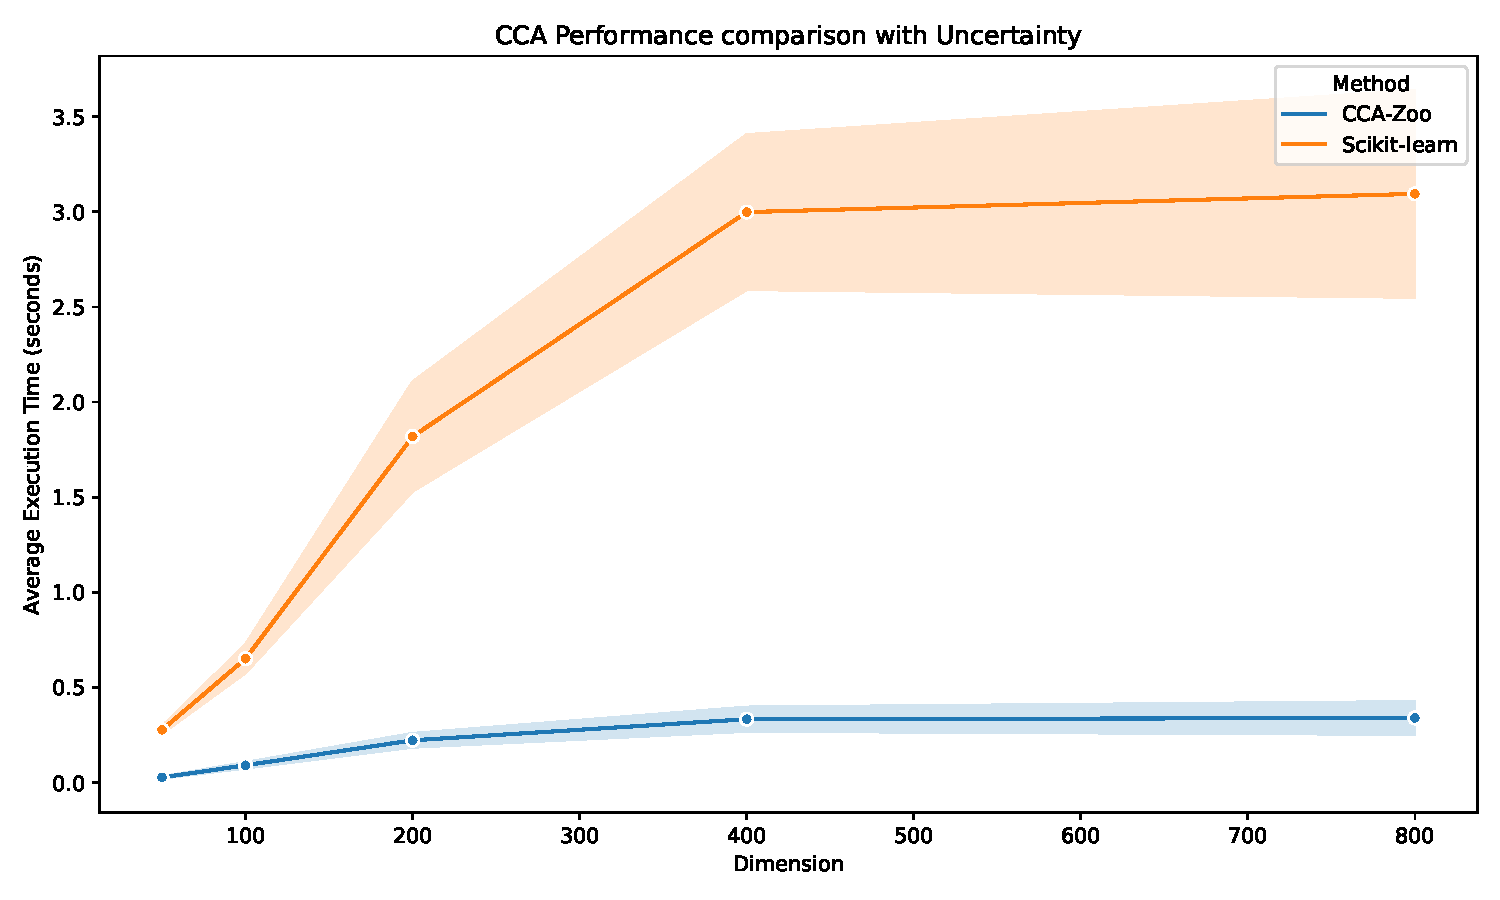
\includegraphics[width=0.9\textwidth]{figures/CCA_Speed_Benchmark}
\caption{Performance comparison for CCA methods}
\label{fig:cca_benchmark}
\end{figure}

The efficiency of \texttt{CCA-Zoo}'s CCA implementation can be attributed to its use of the principal component space for computing the canonical correlations. By first projecting the data onto a lower-dimensional space defined by the leading principal components, \texttt{CCA-Zoo} reduces the computational burden associated with high-dimensional covariance matrices, resulting in faster execution times without sacrificing accuracy.

This performance advantage is particularly relevant in real-world applications, where the number of features often greatly exceeds the number of samples. In such scenarios, \texttt{CCA-Zoo}'s ability to efficiently handle high-dimensional data can lead to significant time savings and enable the analysis of larger datasets.

\subsection{Partial Least Squares}

Figure~\ref{fig:pls_benchmark} shows the execution time comparison for PLS. Similar to the CCA results, \texttt{CCA-Zoo} exhibits a robust performance profile, with execution times that are competitive with those of \texttt{scikit-learn} across all tested dimensionalities.

\begin{figure}[h]
\centering
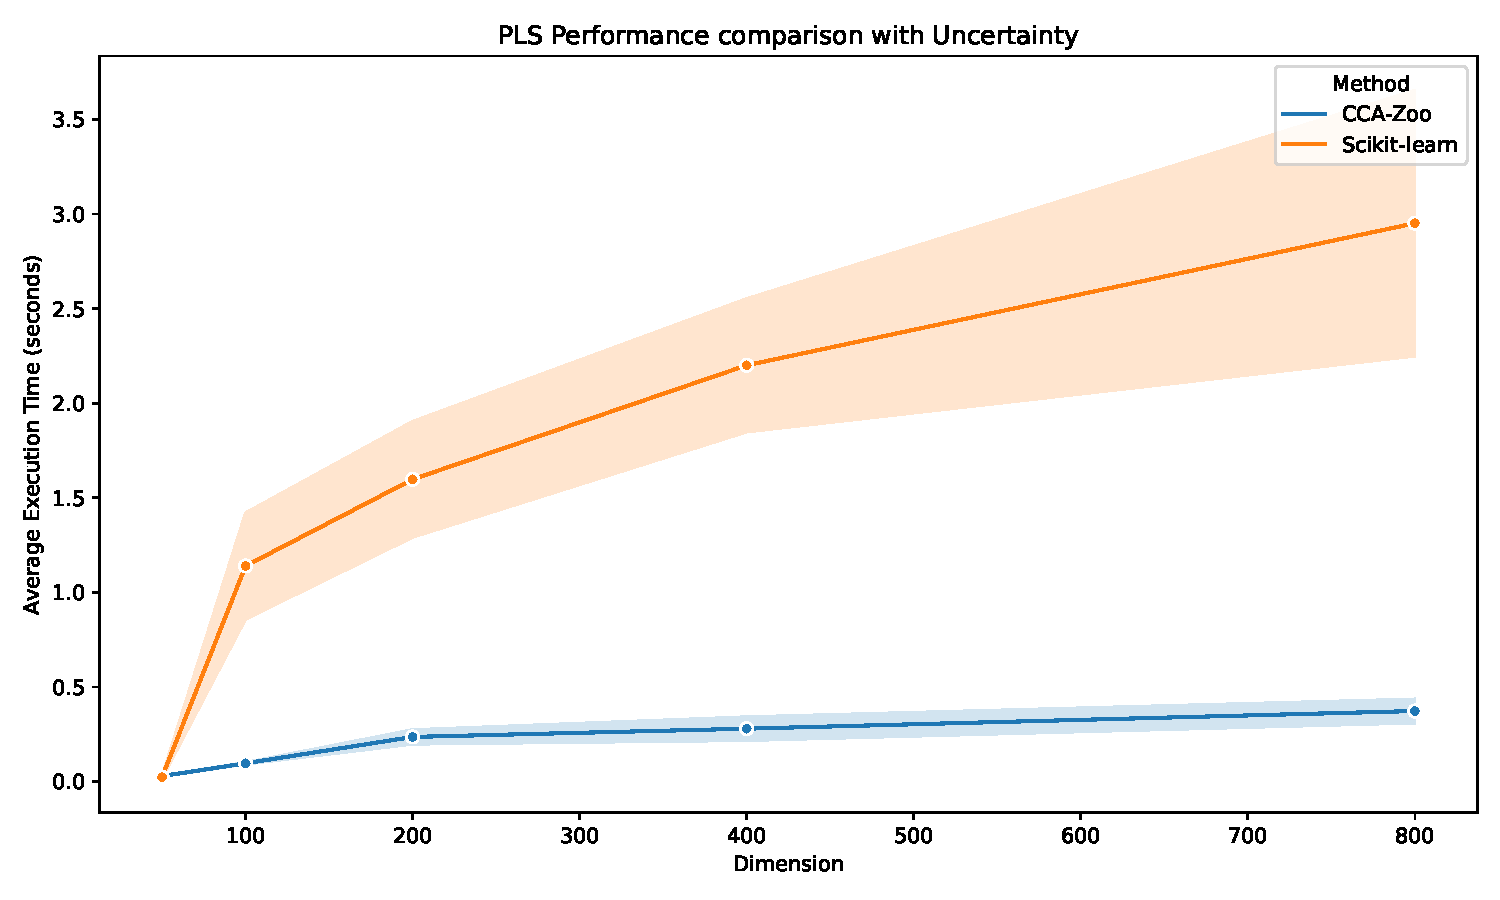
\includegraphics[width=0.9\textwidth]{figures/PLS_Speed_Benchmark}
\caption{Performance comparison for PLS methods}
\label{fig:pls_benchmark}
\end{figure}

The competitive performance of \texttt{CCA-Zoo}'s PLS implementation can be attributed to its use of efficient algorithms and data structures, such as the NIPALS algorithm and the deflation scheme for computing the latent components. These optimizations allow \texttt{CCA-Zoo} to scale well with increasing data dimensionality, making it a suitable choice for a wide range of applications.

\subsection{Real-World Applications}

In addition to the synthetic benchmarking experiments, \texttt{CCA-Zoo} has been used throughout this thesis to evaluate the proposed multiview learning methods on various real-world datasets. These datasets span multiple domains, including bioinformatics and computer vision and pose diverse challenges in terms of dimensionality, sparsity, and noise.

\section{Discussion and Limitations}

\subsection{Contributions and Impact}

The development of CCA-Zoo represents a significant contribution to the field of multiview learning, particularly within the Python ecosystem. By providing a comprehensive and user-friendly library that integrates seamlessly with existing tools like scikit-learn and PyTorch, CCA-Zoo has the potential to greatly accelerate research and application of multiview methods.

Throughout this thesis, CCA-Zoo has played a central role in enabling the empirical studies and method development presented in the previous chapters. The library's efficient implementations of both classical and state-of-the-art multiview algorithms allowed us to conduct extensive experiments on real-world datasets, comparing the performance of different methods and gaining new insights into their behavior. Moreover, the modular design of CCA-Zoo facilitated rapid prototyping and testing of novel extensions and refinements to existing techniques.

Beyond its use in this thesis, CCA-Zoo has already begun to have an impact in the wider research community. The library has been well-received on GitHub, with over 150 stars and 30 forks to date, and has been downloaded nearly 500 times per month from the Python Package Index. Several published papers and ongoing projects in fields ranging from genomics to neuroscience have used CCA-Zoo, demonstrating its potential to enable new discoveries and applications.

\subsection{Limitations and Future Work}

While CCA-Zoo provides a solid foundation for multiview learning in Python, there are certainly areas where it could be improved and extended. One current limitation is the lack of GPU acceleration for some of the more computationally intensive methods, which could hamper their scalability to massive datasets. In future versions, we plan to leverage libraries like cupy to enable seamless GPU support.

Another direction for future work is to expand the library's functionality to encompass an even wider range of multiview learning paradigms, such as multi-modal deep learning, multi-view clustering, and multi-view matrix factorization. By providing a unified interface to these diverse approaches, CCA-Zoo could serve as a powerful toolkit for exploring and combining different perspectives on data.

Finally, we are committed to the ongoing maintenance and development of CCA-Zoo as an open-source project. We welcome contributions from the community in the form of bug reports, feature requests, documentation improvements, and code contributions. By engaging with users and incorporating their feedback, we hope to continuously refine and enhance the library to better serve the needs of multiview learning researchers and practitioners.

\subsection{Conclusion}

In conclusion, CCA-Zoo fills an important gap in the Python ecosystem by providing a comprehensive, efficient, and user-friendly library for multiview learning. Through its extensive catalog of classical and modern multiview methods, seamless integration with popular machine learning tools, and flexible API, CCA-Zoo enables researchers and practitioners to easily explore and apply these powerful techniques to their own data and problems.

The development of CCA-Zoo has been a central contribution of this thesis, underpinning many of the empirical studies and methodological advances presented in earlier chapters. By making the library open-source and freely available to the community, we hope to accelerate progress in multiview learning and promote reproducible, extensible research.

Looking ahead, we see ample opportunities to expand and refine CCA-Zoo, in collaboration with its growing base of users and contributors. Through sustained development and community engagement, we believe CCA-Zoo has the potential to become an indispensable tool in the multiview learning toolkit, enabling new discoveries and applications across a wide range of domains.